\documentclass[a4paper,12pt]{jreport}
%---------------------------------------------------
\usepackage[dvipdfmx]{hyperref}
\usepackage{pxjahyper}
\usepackage{bm}
\usepackage{graphicx}
\usepackage{amssymb,amsmath}
\usepackage{ascmac}
\usepackage{float}
\usepackage{setspace}
\usepackage[dvipdfmx,usenames]{color}
\usepackage{colortbl}
\usepackage{algorithm}
\usepackage{algorithmic}
\usepackage{setspace}
\usepackage{subfigure}
\usepackage{here}
% \usepackage{redeffont}
\usepackage{listings,jvlisting} %日本語のコメントアウトをする場合jvlisting(もしくはjlisting)が必要
\usepackage{booktabs}
\usepackage{titlesec}
\usepackage{siunitx}
\usepackage{array}
%---------------------------------------------------
\definecolor{bl}{rgb}{0.94,0.97,1}
\definecolor{gr}{rgb}{0.5,0.5,0.5}
\makeatletter
\@removefromreset{figure}{chapter}
\def\thefigure{\arabic{figure}}
\makeatother
% \makeatletter
% \def\section{\newpage\@startsection {section}{1}{\z@}{2.3ex plus -1ex minus -.2ex}{2.3 ex plus .2ex}{\Large\bf}}
% \makeatother
%---------------------------------------------------
\setlength{\textwidth}{160truemm}
\setlength{\textheight}{240truemm}
\setlength{\topmargin}{-14.5truemm}
\setlength{\oddsidemargin}{-0.5truemm}
\setlength{\headheight}{0truemm}
\setlength{\parindent}{1zw}
\setlength{\parskip}{0cm} % 段落間
\setlength{\itemsep}{0cm} % 項目間
\setlength{\abovedisplayskip}{1pt}
\setlength{\belowdisplayskip}{1pt}
%---------------------------------------------------
\setstretch{1.0}
%---------------------------------------------------
\renewcommand{\subfigtopskip}{5pt}	% 図の上の隙間。上図の副題と下図の間。
\renewcommand{\subfigbottomskip}{0pt} % 図の下の隙間。副題と本題の間。
\renewcommand{\subfigcapskip}{-6pt}	% 図と副題の間
\renewcommand{\subcapsize}{\scriptsize} % 副題の文字の大きさ
\newcommand{\mysection}[1]{\vspace{-20pt}\section{#1}}
\newcommand{\mysubsection}[1]{\vspace{-20pt}\subsection{#1}}
\newcommand{\mysubsubsection}[1]{\vspace{-10pt}\subsubsection{#1}}
\renewcommand{\lstlistingname}{ソースコード}
\setcounter{tocdepth}{3}
\setcounter{secnumdepth}{3}
%---------------------------------------------------
% ヘッダーとフッターの設定
\usepackage{fancyhdr}
\rhead{\leftmark}
\chead{}
\lhead{\rightmark}
\cfoot{\thepage}

\titleformat{\chapter}% command
    [display]% shape
    {\bfseries\gtfamily\LARGE}% format
    {第\thechapter 章}% label
    {0.5em}% sep
    {}% before-code

\rfoot{}
\begin{document}
%---------------------------------------------------
%ここからソースコードの表示に関する設定
\lstset{
  basicstyle={\ttfamily},
  identifierstyle={\small},
  commentstyle={\smallitshape},
  keywordstyle={\small\bfseries},
  ndkeywordstyle={\small},
  stringstyle={\small\ttfamily},
  frame={tb},
  breaklines=true,
  columns=[l]{fullflexible},
  numbers=left,
  xrightmargin=0zw,
  xleftmargin=3zw,
  numberstyle={\scriptsize},
  stepnumber=1,
  numbersep=1zw,
  lineskip=-0.5ex
}
%ここまでソースコードの表示に関する設定
%---------------------------------------------------
\vspace*{2cm}
\thispagestyle{empty}
\begin{spacing}{1}
\begin{center}
{\Large 明石工業高等専門学校専攻科 \\[1truecm]
専攻科特別研究論文} \\[3.5truecm]
\huge 遠隔型自動運転システムの \\
\huge ユーザビリティに関する研究 \\
\LARGE The Research of Usability of Remote and Autonomous Driving System\\[4truecm]
\Large ME2208 高橋 尚太郎 \\
(機械・電子システム工学専攻) \\[1truecm]
指導教員 野村 隼人
\end{center}
\tableofcontents
\end{spacing}
\pagenumbering{roman}
\newpage
\clearpage
\pagenumbering{arabic}
\pagestyle{fancy}
\setlength{\headheight}{5truemm}


\chapter{序論}
\section{研究背景}

近年、様々な自律移動ロボットの研究開発が行われ、徐々に人間の生活環境に進出し始めている。
従来は、工場における産業用無人搬送車が主体であったが、活躍の場がオフィス、家庭、さらには屋外へと広がりつつある。
今後、ロボットを用いた省力化や危険な仕事の代替を進めるためには、自律移動ロボットが活動できる領域が人間の生活環境へと拡大していくことが期待される。

一例として、自律移動の応用技術として交通課題の解決策として自動運転システムの実用化が進んでいる。現在は法定上遠隔地からの監視・運用を必要とする遠隔型自動運転システムが想定されている。
遠隔型自動運転では、FPV(First Person View)における車速の制御に関して、ドライバの体感速度変化を促すための視覚効果に関する研究が行われている。
視覚効果は、定式化に関して未知数であり、体感速度変化の評価はドライバ自身の知覚の個人差を含めた主観で考えられるため、定性的解析に委ねられている。

自律移動ロボットの実現に関して、工場のように限定された環境では、環境をロボットのために整備することが可能であった。
しかしロボットの活動領域を広げるためには、環境をロボットに合わせて整備するのではなく、ロボットが様々な環境に適応することが求められる。
人間の生活環境は整備された工場と比較して複雑であり、不確実性が高くなる環境である。この不確実性への対処が、重要な課題となる。
特に、ロボットに必要となる知覚、計画、制御のうち、不確実性に最も深く関わるのが知覚(計測と認識)である。
移動ロボットを対象として考えると、重要な知覚の機能として自己位置推定と地図生成(SLAM: Simultaneous Localization and Mapping)がある。
自己位置推定は、ロボットが自身の位置(方位を含む)を認識しながら目的地まで移動するために必要となる。
また地図は、自己位置推定や経路計画に必要である。人手による地図の生成は多大な工数が必要なため、ロボットが自動的に生成することが望ましい。
移動ロボットの自己位置推定と地図生成において不確実性に対処するには、確率論に基づく手法が有効であることが知られている。
確率論に基づくことで、センサデータやコンピュータが持つモデルの不確実性を明示的に表現すると共に、事前確率の情報を用いてより確実性の高い推定を行うことが可能となる。
一般に、SLAMでは、外界センサであるLiDARに加えて、ロータリーエンコーダ、慣性測定ユニット(IMU)等の内界センサによるロボットの移動量の内部情報(オドメトリ)を用いることで、マッピングを行うことが主流とされているが、オドメトリを必要としない、オドメトリフリーのSLAM手法も提案されている。

自律移動ロボットの開発プロセスにおいて、実環境における実証実験が数多く行われている。
特に、屋外における自律移動においては、シミュレーションと実環境では、制約や環境条件が全く異なるため、実環境のみでしか得ることのできない知見が多く、自律移動の実用化に向けては、実機を用いた実証実験が必要とされている。
実証実験に代表されるつくばチャレンジ[1]では、自律移動ロボットの設計において、要素技術であるLiDARを中心とした、センサ系の使用が主となり、複数のセンサとの融合(センサフュージョン)による環境認識の高精度化が図られている。
それと同時に、自律移動ロボットの実用化に向けて、使用されるセンサの選定、用途に応じて最適化する試みが行われている。
特に、ロボットに搭載するセンサの使用数を少なくすることは、ロボットに課される制約・条件、ソフトウェア開発の工数減、保守性の向上のために、考慮すべき点と述べられている。
自律移動チャレンジの参加車両の形態は多様であり、差動二輪型が一般的であるが、パーソナルビークル等の使用としては、4輪車両型の自律移動等も見られる。
自律移動ロボットは、歩行者等と同じ空間に共存するロボットとしての位置づけであり、比較的低速であることが特徴であり、LiDARによる環境認識の比重が高い。
対して、自動運転では、リアルタイム性が重視され、カメラや深度センサ等のイメージセンサ等のコンピュータビジョンとLiDARセンサによるSLAMがそれぞれ同じ割合での併用が標準となり、センサ融合に関する技術について言及されている。

\section{本研究の目的と特徴}
本研究では、ROS\verb|(Robot Operating System)|
を用いた4輪車両型自律移動ロボットシステムの開発を目的として、一つ目に、LiDARのみによるSLAMによって生成された環境地図の評価と、二つ目にステアリングコントローラによる、ハンドルフットペダル型インターフェースによる遠隔操作を用いた、手動運転自動運転の切り替えシステムの開発を行う。
ROSに実装されたSLAMメタパッケージである、
slam\_gmapping
による環境地図構築とNavigationメタパッケージである、Navigation Stack を用いて、Waypoint Navigationにより、中継目的地を経由して、
最終目的地まで自律移動を行い、最終目的地に到着した時点で、手動運転に切り替えることで、運転操作の引継ぎを実現するシステムを構築する。
三つ目に、遠隔型自動運転システムのFPV操作に着目した、自動車の映像における、運転視野角や、映像画角の変化による体感速度のモデルの定量化を目的として、体感速度モデルの定式化を提案する。
自律移動ロボットの要素技術として用いられているLiDARのメーカーとして有名な北陽電機株式会社は、中之島チャレンジに参加し、自律移動ロボットの実機を開発して、実際にフィールドで議論を行うことで、新製品の開発を行っている。
自律移動ロボットの要素技術であるLiDARの開発においても、実証実験が不可欠である。
筆者は、中之島ロボットチャレンジを観戦することで、将来的に自律移動ロボットやLiDARの開発に携わりたいと考えた。
今回は、縁あって北陽電機株式会社様よりLiDARを貸与頂き、有効活用して筆者自らの開発アイデアを実現することを目標として研究に取り組むこととした。
本研究の位置付けは、LiDARの使用技術の勉強並びに、北陽電機株式会社様への就職を目的としている。

\section{本論文の構成}

本論文は全5章から構成される。以下に各章の概要を述べる。

第1章では、本研究の背景と目的及び各章の構成を述べた。

第2章「FPV車両操作の体感速度変化率の定式化」では、ドライバの体感速度変化を促すための視覚効果に関する仮説を提案する。具体的には、体感速度の変化率を支配するパラメータに着目し、走行映像の視聴環境ドライバの視野角と、走行映像のクロップ率をパラメータとしたときの単位時間当たりの映像ピクセルの移動量を体感速度の変化率として、クロップ率・視野角の減少と増加の特性を一つのモデルとして定式化した。

第3章「LiDARのみのSLAMにより作成された環境地図の評価」では、内界センサによるオドメトリを用いず、ROSで実装されている各LiDAR SLAMパッケージを用いたLiDARのみによる環境地図作成システムを開発し、オドメトリフリーの手法に対して、オドメトリが必要な手法にLiDARから得るレーザオドメトリを用いて比較することで、LiDARのみによるSLAMの性能を明らかにした。

第4章「自動運転システムの開発」では、測距センサ(LiDAR)による測距データのみを用いたSLAMによって作成された環境地図を用いて、4輪車両型RCカーのLiDARのみによる自己位置推定とWaypoint Navigationの有用性の検証を行った。特に、4輪車両特有の動作である、切り返しの実現性、自動運転システムとして機能をする場合の遠隔操作のユーザビリティと、手動・自動運転のタスクの切り替え機能の動作に着目をした評価を行った。

第5章「結論」では、本研究で得られた結果とその成果について述べる。


\chapter{FPV車両操作の体感速度変化率の定式化}
\section{はじめに}
体感速度の変化とは、基準となる速度に対して、観測環境における何らかのパラメータの作用により、視覚的な体感情報から得られる速度感覚が基準と比べて変化する現象のことである。
自動車を運転する際、車速の増加によってドライバの有効視野角が狭まり、ドライバの体感速度が減少する現象が報告されている。
また、低速状態においても、ドライバの視野角の変化、運転視野映像のクロップによって体感速度が変化する現象が一般的に知られている。
また、自動車等を、カメラ映像を確認しながら遠隔操作(FPV:First Person View操作)する際に、カメラの設定によって同様の現象が起こる。
これはカメラ映像による視覚情報が、遠隔操作を行うための操作者への体感情報に影響を与えるためだと考えられている。
具体的には、カメラの画角の設定などが挙げられる。FPVは、操作対象から見た視点であり、操作者が操作対象から周囲の景色を見ることを目的としている。
自動車の運転操作と、遠隔型自動運転や、FPVによるRCカーの操作では、スケールの違いや、カメラの画角の設定等から、視覚情報から得られる体感情報において矛盾が生じる。
一例として、操作対象自身の視点から体感する感覚的な移動速度(体感速度)を錯覚する。
一般に、自動車のドライバが利用する情報のおよそ 90\%が 視覚情報であると報告されており、ドライバが受け取る情報の大部分を占めているため、体感速度の錯覚が、適切な運転に影響を与え、思わぬ事故を引き起こす恐れがある。
体感速度の錯覚は、走行環境と自動車の運転速度の変化によっても生じる。より広い道路を高速で移動すると、人間の視野における周辺視の減少により、自動車の体感速度を実際の速度よりも低く感じるように錯覚すると報告されている。
高速道路等で体感速度を低く感じると、ドライバは、車速を増加させる傾向にある。車速の増加が自動者事故の原因になる。
また、逆に低速域においても視野角の減少によって体感速度が減少することが報告されている。また、ゲーム等の演出で使用されているものとしては、視野を広げると速く見せることができる。
一方、運転映像や運転中の視野角の変化による体感速度の比率の定量化に関しては行われていない。視野角を狭めることによる効果や、視野の増加によって得られる体感速度の定量化\verb|(モデル化)|はされていない。
また、視野角の減少と増加の両方における体感速度の変化を一つの特性として表した例はない。
体感速度を定式化することができれば、映像から得られる視覚効果の影響を光学的に応用し、FPV操作や、ヘッドアップディスプレイ等によって、ドライバの体感情報の補正手法としての応用が期待できる。
そこで我々は、自動車の映像における体感速度のモデルの定量化を目的として、体感速度モデルの定式化を提案する。
DSの走行映像において観測者の体感速度の減少を促す映像クロップと視野角の特性を求め、クロップ率-体感速度と、視野角-体感速度の幾何学モデルを定式化する。
本研究では、クロップ率・視野角の減少と増加の特性を一つのモデルとして表し、視野角の変化に対する体感速度の変化を定式化することで、映像から得られる体感速度を定量的に定義した。

\section{従来研究}
淺田ら\cite{taikan:asada}は、人間の視覚情報を用いた体感速度変化を利用した研究として、ドライビングシミュレータの操作視点にバーチャルパターンを投影することによって、ドライバに適切な速度制御を促す手法が提案されている。
運転者の速度制御をモデル化することにより、ドライバが適切な速度を制御できない要因として「環境からの速度認知に関する誤差が大きいこと」、「目標速度設定が適切でないこと」の2点が挙げられることを明らかにした。
前者の要因を改善するバーチャルパターンとして、一定速度で移動するバーチャルパターン、流れる風景を誇張表現するバーチャルパターンを挙げ、バーチャルパターン投影映像の視聴実験の被験者の主観評価により、これらの有効性を確認した。
これらは、目標速度制御のための定性的な効果であり、体感速度の変化に寄与するパラメータについては言及されておらず、体感速度の変化を示すものは、被験者の主観による評価であるため、視覚効果の定量的な評価はされていない。

大前ら\cite{taikan:ohmae}は、遠隔操縦に基づく資格情報の影響を評価し、遠隔操縦において、カメラ条件や映像条件が運転操作に与える影響を評価している。評価結果に基づいて遠隔操縦車両および、その制御系を構築し、遠隔操縦と直接運転を比較することで、本研究で構築した遠隔操縦システムの構成により、直接運転と近い運転操作が実現できることを明らかにした。
視覚情報の影響評価においては、カメラの視野角の影響が大きく、フレームレートや解像度などの影響が相対的に小さいことが報告されている。
以上より、遠隔操縦における視覚情報の運転への影響として、視野角による影響が大きいことが述べられている。

Speed Management \cite{taikan:speedmanagement}によると、速度が上がるとドライバの視野が狭くなることが報告されている。
時速40 km の場合、ドライバの視野は 100度であり、路傍の障害物やその他の潜在的な危険を確認できる。図\ref{taikan:speed}に視野角と体感速度の関係を示す。
時速 130 km では、視野は約 30°にまで減少し、ドライバが潜在的な危険を判断する能力が大幅に低下するとされている。

\begin{figure}[h]
  \begin{center}
  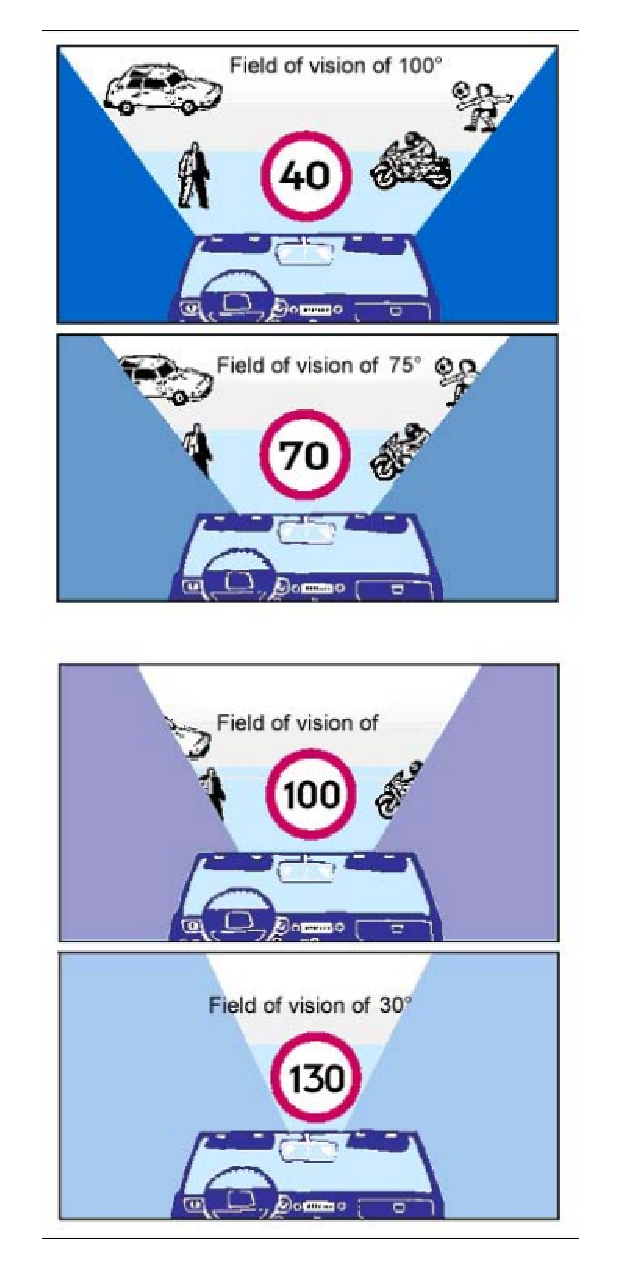
\includegraphics[width=.5\linewidth]{img/1.eps}
  \caption{視野角と体感速度の関係\cite{taikan:speedmanagement}}
  \label{taikan:speed}
  \end{center}
\end{figure}

\clearpage
体感速度を支配するパラメータとして、運転者の速度に影響を与えるパラメータに関する研究をいくつか述べる。

AR 技術を用いて運転者の体感速度を変化させる試みとして東井ら\cite{taikan:higashii}は単純な線や四角形からなるパターン の速度を実際よりも速く表示することで運転者の体感速度を変化させることに成功していた。しかし、実際にどのような速度制御が行われるかや他の表示方法で表示した場合の効果は未知数である。

走行速度と道路環境の関係についての調査として Gitelman\cite{taikan:gitelman}らは運転者が速度超過する原因は道路環境から人々が適切と感じる速度と制限速度があっていないこととし, どういった要素が適切と感じる速度に影響を与えているかを実際の道路環境の要素の調査と運転者への意識調査によって検証した。結果として視野的狭窄や歩行者の活動、道路のレイアウト等が要素として挙げられることが分かった。

Joら\cite{taikan:jo}は、運転速度がドライバの視覚的注意に及ぼす影響を、ドライバが処理できる視覚情報の最大量とのバランスがとれる最大視野という観点から評価を行った。
運転速度の増加により、処理する視覚情報の量が増加するため、ドライバが処理する視覚情報の量が、自身の取得できる最大量と釣り合う点までしか視野を広げることができないとした。
この点を超えるとドライバは、不安、ストレスの増加によりドライバが取得できる最大の視覚情報が減少し、視野がさらに狭くなって心理的圧迫感を感じる現象(トンネル効果)が起きる可能性があると述べている。具体的に、ドライバは、潜在的な危険があった場合に対処するための時間を確保するために、運転速度が上がるにつれて遠くを見る傾向がある。 これは、運転速度の増加による流体刺激の増加だけでなく、遠くを見ることでの視野の増加により、ドライバが処理する視覚情報の量が増加し、ドライバの精神的負担が増大することを意味する。ドライバは、安全を確保するために、取り扱える視覚情報の量が許される限り、可能な限り多くの視覚情報を取得する傾向にある。しかしながら、前述したように、運転者が取り込める最大の視覚情報は、運転の専門知識のレベルに応じて個人差がある。走行速度が取り込める視覚情報の許容量が釣り合う点を超えた場合、ドライバは自動的に視野を狭めることで視覚的情報の許容が釣り合う点を自己維持しようとし、処理する視覚情報の量を減らす。
一部のドライバにとっては、バランス点を超える不安ストレスが非常に高くなり、バランス点を超えた後に処理できる最大の視覚情報がさらに減少するとしている。

\section{体感速度のパラメータの模索}
RCカーと実車の速度が視覚的に一致すること(体感速度が一致すること)を目的として、体感速度の変化を及ぼすパラメータを、RCカー・DSの走行映像の比較により調査した。体感速度の比較について、車両模型の迫力・臨場感の表現として用いられるスケールスピードとの比較も行った。これにより体感速度の一致の目標が、走行映像中における単位時間当たりの描画の移動ピクセル数の一致であることが分かった。また、この目標を達成するためのパラメータを明らかにした。

\subsection{原理}
図\ref{taikan:genri}に、体感速度の原理を示す。
一般に、トラックなど乗用車よりも車高が高くなる車両を運転する場合、体感速度は遅くなり、
逆に、レースカート等の車高の低い車両を運転すると体感速度は速く感じる。RCカーを運転する場合は後者に相当する。その原理を幾何学的に説明する。

\begin{figure}[h]
  \begin{center}
  \includegraphics[width=.95\linewidth]{img/2.pdf}
  \caption{体感速度の原理}
  \label{taikan:genri}
  \end{center}
\end{figure}

体感速度の変化は上下・左右方向の視野それぞれの影響が存在する。
一例として上下方向の視野の場合を説明する。操作視点が高い時の視点は、低い時の視点の延長線上にある。
ある点から他方の点まで進んだ時も同様になる。実車あるいはRCカーが、体感的と同じ速度で移動しているための条件は、画面上のピクセルの移動速度(実際の線を移動する時間)が、実車とRCカーで同じになることである。
RCカーと実車で速度が同じでも、風景が移動する速度が異なるために体感速度が異なる。
このRCカーの実速度に対して体感速度が同じになる実車の速度との比を求めることで、体感速度の一致を求めることができる。
つまり、体感速度の一致を走行映像中の単位時間当たりの移動ピクセル数の一致とする。

\subsubsection{体感速度とスケールスピードについて}
スケールスピードとは、模型車両の実際の移動速度にスケール比の平方根を乗じたものを、実際の車両のスケールでの速度としたものである。
実際の速度にスケール比を乗ずるのではなく、力学的な相似効果から迫力の表現として使用されている。
スケールスピードの導出には、流体分野における流れの相似の指標とするフルード数が用いられ、以下のようにして導出する。

フルード数$Fr$の定義は、式\eqref{taikan:eq:frude}で表される。

\begin{align}
  Fr = \frac{U}{\sqrt{Lg}} \label{taikan:eq:frude}
\end{align}

ここで、$U$:体感速度\si{[m/s]}、$L$:代表長さ\si{[m]}、$g$:重力加速度\si{[m/s^2]}である。実車の特性速度、代表長さをそれぞれ、
$U_1$、$L_1$、RCカーの特性速度、代表長さを$U_2$、$L_2$とすると、それぞれが力学的に相似であることから、フルード数が一致するという条件のもとで、
立式すると式\eqref{taikan:eq:frude2}、\eqref{taikan:eq:frude3}のようになる。

\begin{align}
  \frac{U_1}{\sqrt{L_1g}} = \frac{U_2}{\sqrt{L_2g}} \label{taikan:eq:frude2}\\
  U_2 = \frac{U_1}{\sqrt{\frac{L_1}{L_2}}} \label{taikan:eq:frude3}
\end{align}

$\frac{L_1}{L_2}$は、実車とRCカーのスケール比であるため、特性速度、$U_2$がRCカーのスケールスピードであり、実車の速度$U_1$をスケール比の平方根で除すると求めることができる。

\subsection{DS・RCカーの走行映像の解析}
ここでは、DSとRCカーの走行映像の比較について述べる。
DS上の実速度とRCカーのスケールスピードが一致する場合RCカーと実車の体感速度が等しいと仮定して、
RCカーとDSの走行映像の単位時間あたりの移動ピクセル数の一致を目指す。またスケールスピードではなく、スケール比を乗じた速度での走行映像との比較も行った。

\subsubsection{実験方法}
\begin{enumerate}
  \item RCカーの走行環境を作成する。図\ref{taikan:rc}に、RCカーの走行環境を示す。今回は移動ピクセル数の比較のために、コース車両の脚部分に黄色い装飾を施した。RCカーに設置したカメラで定速走行映像を撮影し、始点・終点間の動画の再生時間で除して実速度を求め、スケール比の平方根との積によりスケールスピードを計算する。RCカーの移動速度は、RCカーのDCモータのPWM制御によって行われているため、PWM周期の入力値と出力値を実測する。この出力値を用いてRCカーの移動速度を計算している。
  \item DS上で実車スケールのRCカーの走行環境を作成する。図\ref{taikan:ds}にDS上で再現したRCカーの走行環境を示す。RCカーの現物の環境と視覚的な条件を等しくするために、RCカーの走行実験で使用した環境の壁面\verb|(机)|の寸法を測定し、走行路面をテクスチャマッピングによって再現した。
  \begin{figure}[h]
    \begin{center}
    \subfigure[RCカーの走行環境]{
    \includegraphics[width=.4\columnwidth]{img/3.jpg}
    \label{taikan:rc}
    }
    \subfigure[DS上で再現したRCカーの走行環境]{
    \includegraphics[width=.52\columnwidth]{img/4.png}
    \label{taikan:ds}
    }
    \caption{体感速度の実験環境}
    \label{taikan:jikken1}
    \end{center}
  \end{figure}
  \item DSの走行環境においてRCカーのスケールスピードで走行した映像を撮影する。DSとRCカーの走行映像を見比べて、単位時間当たりに通過するポールの数を目視で確認し、スケールスピードと体感速度の一致・不一致を評価する。
  \begin{figure}[h]
    \begin{center}
    \includegraphics[width=.88\linewidth]{img/5.jpg}
    \caption{単位時間当たりに通過するポールの数の確認}
    \label{taikan:pall}
    \end{center}
  \end{figure}
  \item RC映像にスケール比を乗じた速度のRCカーの走行映像を取得する。
  \item スケールスピードでの比較とスケール比をかけた速度を比較する。
  \item 体感速度が一致しない場合、その原因を検討し、パラメータとする。
\end{enumerate}
なお、本実験で作成したDS環境の寸法を図\ref{taikan:dsm1}、\ref{taikan:dsm2}に示す。DS上の環境に関しては、RCカーのスケール比に合わせて作成した。
今回用いたRCカーのスケールが$\frac{1}{10}$であったため、実際のRCカーの走行環境を10倍したDS上の走行環境とした。

\begin{figure}[h]
  \begin{center}
  \subfigure[DS上コースの寸法:全体]{
  \includegraphics[width=.8\columnwidth]{img/6.png}
  \label{taikan:dsm1_1}
  }
  \subfigure[DS上コースの寸法:全長]{
  \includegraphics[width=.8\columnwidth]{img/7.png}
  \label{taikan:dsm1_2}
  }
  \caption{DS環境の寸法:全体}
  \label{taikan:dsm1}
  \end{center}
\end{figure}

\begin{figure}[h]
  \begin{center}
  \subfigure[DS上コースの寸法:障害物]{
  \includegraphics[width=.8\columnwidth]{img/8.png}
  \label{taikan:dsm2_1}
  }
  \subfigure[DS上コースの寸法:道幅]{
  \includegraphics[width=.8\columnwidth]{img/8.png}
  \label{taikan:dsm2_2}
  }
  \caption{DS環境の寸法:詳細}
  \label{taikan:dsm2}
  \end{center}
\end{figure}

実験の様子を図\ref{taikan:hikaku}に示す。
今回のスケールスピードの比較は、表に示す32\verb|~|48 \si{[km/h]}
の6パターンで行った。一例として、RCカーのスケールスピード32 \si{[km/h]}(実際の速度は10\si{[km/h]})とDS上の速度32\si{[km/h]}の比較を行う。

スケール比での比較は、RCカー の実際の速度10 \si{[km/h]}とDSの100 \si{[km/h]}の映像で行った。
体感速度の評価を目的としてDSとRCカーの走行映像をPCディスプレイ上に並べて視聴する。
視聴者の主観によって体感速度の遅速・一致を評価する。体感速度が一致しない映像を観察することで、体感速度の変化を示すパラメータを模索する。

\begin{figure}[h]
  \begin{center}
  \includegraphics[width=\linewidth]{img/10.png}
  \caption{実験の様子}
  \label{taikan:hikaku}
  \end{center}
\end{figure}

\clearpage
\subsubsection{実験結果}
実測値とスケールスピードの計算結果を表\ref{taikan:table1}に示す。RCカーのスピードはモータの回転数を回転数計で計測し、
計算を行って、時速への変換を行っている。なお、モータの回転数は10回計測した際の平均値を採用している。
 
\begin{table}[ht]
\centering
\caption{実速度とスケールスピードの計算結果}
\scalebox{.83}{
\begin{tabular}[t]{rrrrrr}
\toprule
パルス入力値\si{[\micro s]}&パルス測定値\si{[\micro s]}&パルス誤差&回転数\si{[rpm]}&実速度\si{[km/h]}&スケールスピード\si{[km/h]}\\
\midrule
1348&1329&19&2194&24.81&78.47\\
1402&1386&16&1896&21.44&67.81\\
1438&1418&20&1589&17.97&56.83\\
1458&1440&18&1337&15.12&47.82\\
1480&1460&20&1161&13.13&41.52\\
1502&1482&20&854.6&9.666&30.57\\
\bottomrule
\label{taikan:table1}
\end{tabular}}
\end{table}%

モータの回転数を時速に変換する式を式\eqref{taikan:eq:motor}に示す。
\begin{align}
  v_{km} = d \times r \times 0.01885 \label{taikan:eq:motor}
\end{align}
ここで、$v_{km}$:時速、$d$:ホイールの直径\verb|(|6 \si{[cm]}\verb|)|、$r$:回転数\si{[rpm]}、\\0.001885:係数成分:$\frac{3600}{1000}\times\frac{2\pi}{60\times100}$
である。

RCカーのスケールスピード32 \si{[km/h]}\verb|(|実際の速度は10 \si{[km]}\verb|)|とDS上の速度32 \si{[km/h]}で比較した場合は、体感速度が一致しなかった。RCカーの速度10 \si{[km/h]}とDS上の速度100 \si{[km/h]}を比較した場合は、体感速度が一致した。
実験結果より、RCカーの操作視点カメラ映像の方が、DSの操作映像よりも体感速度が速いと評価されるため、RCカーのスケールスピードは体感速度と一致しないことを確認した。また、スケール比で走行させた場合に体感速度が一致したことから、
RCカーと自動車における移動ピクセル比は、スケール比の平方根ではなく、スケール比と同じ値をとることが検証された。
つまり、体感速度は、スケールスピードによる力学的相似ではなく、単純なスケール比を一致させた場合に一致すると言える。
次に、スケールスピードと体感速度が一致しない原因として検討したパラメータを挙げる。

\begin{enumerate}
  \item 映像中の風景線が流れるスピード\verb|(映像ピクセルの移動速度)|\\
  撮影範囲の道路における白線や、壁面と空との境界線等の風景線が単位当たりに移動する映像上でのピクセル数に注目することで、体感速度が異なることを確認した。
  \item 地上高\\
  RCカーの方が、実車と比べて操作視点の地上高が低いため、近くを見るようになる。景色は遠くより近くの方が速く流れるため、体感速度が上がる。これは、電車に乗って外を見ると、近くの建物は速く動くが、
  遠くの山などは遅く動くことと同じ現象である。RCカーの操作視点カメラの取り付け位置を変更し、変更前の走行映像と比較したが、体感速度に変化は見られなかった。
  \item 水平線に対する地面の割合\\
  地上高が低くなり、近くを見るようになることで、水平視点に対して、地面が見える割合が増えることによって体感速度が上がると推測した。水平線に対する地面の割合を変えるために、カメラの下半分を段ボールで隠し、
  水平線以上の景色のみしか撮影できないようにすることで、早く流れる近くの景色を遮断し、遠くの景色のみを写す。これによって体感速度を変化させる効果は得られなかった。
  \item 操作映像のクロップ・カメラの画角\\
  RCカーの操作視点カメラ映像を拡大クロップすることで、RCカーの体感速度が減少し、DSの映像とおおよそ一致したことを確認した。カメラ映像の画角体感速度の抑制に最も大きな効果を与えた。また、映像のクロップは、カメラ映像の画角を狭くする\verb|(|カメラの種類を広角・狭角と変更する\verb|)|ことと同じ効果を得ることができた。
\end{enumerate}

\subsection{体感速度のパラメータの選定}
前で述べた体感速度のパラメータのなかで影響度が高いものを選定する。映像のクロップ率を変化させることで、他の全てのパラメータが変化し、体感速度の中で最も影響の高いパラメータであることが明らかになった。

\subsection{映像のクロップによって体感速度変化を促す方法}
本実験で使用したカメラは水平視野角が120度である広角レンズを使用している。
このため、体感速度が実際よりも早く感じることがあった。カメラの種類\verb|(狭角・広角)|を変えることは容易ではないが、
撮影映像を編集することで体感速度を変化させる方法について検討した。その結果、映像をクロップ\verb|(映像の一部を拡大表示)|して画面全体に表示させることで、
元の映像よりも体感速度を減少させる効果を得た。

\subsubsection{映像のクロップ手法}
図\ref{taikan:crop1}、\ref{taikan:crop2}に映像クロップの概要を示す。以下にクロップの手順を示す。
\begin{enumerate}
  \item FPV映像をクロップし、元の解像度の比となるように拡大する。
  \item 拡大クロップしたRCカーの車体が見える部分\verb|(下部)|を削除する。
  \item 拡大クロップした映像の上部1を、DSの映像における水平消失点の流れと合わせるように切り取る。
  \item 拡大クロップした映像の残った部分を削除し、流れを合わせるように切り取った上部映像を、下部と繋がるように位置を下げる。
  \item 1の上部と連続している映像2を下のFPV映像から切り取る。
  \item 1の上部に2を繋ぎ合わせる。
\end{enumerate}

\begin{figure}[h]
  \begin{center}
  \includegraphics[width=.8\linewidth]{img/8_1.jpg}
  \caption{クロップ手順1}
  \label{taikan:crop1}
  \end{center}
\end{figure}

\begin{figure}[h]
  \begin{center}
  \includegraphics[width=.9\linewidth]{img/8_2.jpg}
  \caption{クロップ手順2}
  \label{taikan:crop2}
  \end{center}
\end{figure}
\clearpage
この実験によって、変化したパラメータについて述べる。クロップ率を増加させることで、映像の縦横の長さが減少し、視野角が減少することが明らかになった。
また、そのほかのパラメータも同時に変化し、クロップ率・視野角が体感速度の変化を制御するパラメータであることを定性的に示した。この時点では定量的な解析はできない。

\subsection{映像クロップによる体感速度の変化の仮説}
クロップ率の変化によって、体感速度が補正される根拠を以下に示す。
\begin{enumerate}
  \item 地上高\\
  手元の景色を排除し、遠くの景色を拡大したため、遠くの景色の流れが遅くなることから、体感速度が遅くなる。
  \item ピクセル\\
  映像のクロップにより、近くに見える映像がより遠い位置になるため、水平面より下の景色の流れが遅くなることで、ピクセルの移動速度が遅くなり、体感速度が遅くなる。
  \item 水平面より下の景色\\
  図\ref{taikan:cropzengo}にクロップ前後の見え方の変化について示す。

  \begin{figure}[h]
    \begin{center}
    \includegraphics[width=.8\linewidth]{img/9_1.pdf}
    \caption{クロップ前後の見え方の変化}
    \label{taikan:cropzengo}
    \end{center}
  \end{figure}
  映像のクロップにより、クロップ前に見えていたものが前進する。それにより、見かけ上の位置がクロップ前と比べて、近くに見える映像がより遠い位置になるため、水平面よりも下の景色の見え始めが遠くなる。
よって、水平面より下の景色の流れが遅くなることで、体感速度が遅くなる。
\end{enumerate}

本研究以外にも同様の報告として、論文によると、映像のクロップによる体感速度の増強効果が、報告されている。
また、レース用ゲーム等で用いられる手法として取り入れられていることを確認している。

\clearpage

\subsection{体感速度のパラメータの導入}
体感速度変化で最も影響力のあるパラメータが映像のクロップとカメラの画角であることが分かった。
一般的に、走行映像を投影するカメラの画角に加えて、車両のドライバの視野角の変化が体感速度変化に寄与すると考えられている。
また、映像のクロップによってカメラの画角の変化が可能であることが共通の見識として共有されている。
つまり、映像のクロップによって、容易に車両中のドライバの視点の視野角を変化させることができ、体感速度を変化させることができる。
しかし、映像のクロップでは、ドライバの視野角を縮小する場合のみでしか検証ができない。
DSの視野角変更機能を用いることで、カメラの画角・ドライバの視野角を拡大する場合の検証を行うことができる。
そこで、本研究では、画角(視野角)・クロップというパラメータを導入し、映像のクロップを拡張し、
ドライバの視野角の拡大における体感速度の変化に関しても検討を行う。


\section{体感速度モデルの提案}
これまで、スケールスピードと実速度を比較することで、体感速度はスケールスピードと一致せず、単なるスケール比に一致することが明らかになった。
さらに、その過程において体感速度を変化させるパラメータを発見した。列挙した中で最も影響力のあるパラメータが、走行映像のクロップ率やカメラの画角・ドライバの視野角であることが明らかになった。
そこで、走行映像のクロップ率とドライバの視野角を体感速度変化のパラメータとして、体感速度を定式化する手法を提案する。本研究では、実測値との比較として、視野角・ディスプレイ比等、DS環境におけるパラメータを定数とした
幾何学計算による幾何学モデルを提案する。

\subsection{原理}
実車が同じ速度で走行する場合でも、視野角が広い方が、体感速度が速く感じるという現象が生じる基準視野角と、ある視野角での画面上の一方から他方の点にかけてのピクセルの移動距離の比が体感速度の比となる。
図\ref{taikan:pixel}に、ピクセルの移動距離の考え方を示す。
同様の原理として、交通事故で取り上げられるコリジョンコース現象が挙げられる。複数の走行映像において、ピクセルの移動速度が一致する時、体感速度の比と一致していることが望ましい。

\begin{figure}[h]
  \begin{center}
  \includegraphics[width=.65\linewidth]{img/11.jpg}
  \caption{ピクセルの移動距離の考え方}
  \label{taikan:pixel}
  \end{center}
\end{figure}

\clearpage
\subsection{体感速度モデルの定式化}
体感速度を求めるために、映像中のポール間の移動の際に映像中の移動ピクセル数と、環境によって決まるパラメータを定式化する。
ここでは、体感速度$v_{sense}$を、視野角の関数$f(h_{fov_v})$で表し、$h_{fov_v}$を、クロップ率の関数$g(n)$で表すことを目標とする。
実際の速度\verb|(実速度とする)|を$v_2$とすると、式\eqref{taikan:eq:model1}、\eqref{taikan:eq:model2}に示す関係式を求める。

\begin{align}
  v_{sense} = f(h_{fov_v})\cdot v_s = f(g(n))\cdot v_s \label{taikan:eq:model1}\\
  h_{fov_v} = g(n) \label{taikan:eq:model2}
\end{align}

まず、ディスプレイのアスペクト比とサイズ(ディスプレイの対角線の長さ)をディスプレイの縦・横の長さに変換する式を式\eqref{taikan:eq:dis1}、\eqref{taikan:eq:dis2}に示す。図\ref{taikan:displaytosize}
にディスプレイ長さの概要と諸条件を示す。

\begin{figure}[h]
  \begin{center}
  \includegraphics[width=.65\linewidth]{img/12.pdf}
  \caption{ディスプレイ長さの概要と諸条件}
  \label{taikan:displaytosize}
  \end{center}
\end{figure}

\begin{align}
    D_v = D_{ch} \cdot m \cdot \frac{b}{\sqrt{a^2+b^2}} \label{taikan:eq:dis1}\\
    D_h = D_{ch} \cdot m \cdot \frac{a}{\sqrt{a^2+b^2}} \label{taikan:eq:dis2}
\end{align}

$D_v$:ディスプレイの縦の長さ\si{[cm]}、$D_h$:ディスプレイの横の長さ\si{[cm]}、$D_{ch}$:ディスプレイの対角線の長さ\si{[inch]}、
$m$:2.4\si{[cm/inch]}、$a$:ディスプレイの横のアスペクト比:16、$b$:ディスプレイの縦のアスペクト比:9とする。

次に、ディスプレイの縦・横の長さとディスプレイとの視点距離をDS上での水平・垂直方向の基準視野角に式\eqref{taikan:eq:kijun1}、\eqref{taikan:eq:kijun2}を用いて変換する。
図\ref{taikan:kijuntods}に基準視野角とその導出の諸条件を示す。


\begin{figure}[h]
  \begin{center}
  \subfigure[水平方向]{
  \includegraphics[width=.4\columnwidth]{img/13_1.pdf}
  \label{taikan:kijuntods1}
  }
  \subfigure[垂直方向]{
  \includegraphics[width=.52\columnwidth]{img/13_2.pdf}
  \label{taikan:kijuntods2}
  }
  \caption{基準視野角とその導出の諸条件}
  \label{taikan:kijuntods}
\end{center}
\end{figure}

\begin{align}
    h_{fov_s} = 2\arctan{\frac{D_h}{2f}} \label{taikan:eq:kijun1}\\
    v_{fov_s} = 2\arctan{\frac{D_v}{2f}} \label{taikan:eq:kijun2}
\end{align}

$h_{fov_s}$:基準水平視野角\si{[degree]}、$v_{fov_s}$:基準垂直視野角\si{[degree]}、$f$:視点距離\si{[cm]}とする。

次に、基準視野角を映像クロップによる視野角に変換する。クロップ率$n$の値域は、$1 \leqq n \leqq 3.5$とする。
$n = 1$の時$h_{fov_s}$、$v_{fov_s}$(基準視野角)とする。
式\eqref{taikan:eq:crop1}、\eqref{taikan:eq:crop2}は、映像のクロップにより、視野範囲が変わることを意味する。
クロップは縦横比を一定とし、映像の中心は変化させない。図\ref{taikan:shiyatocrop}に映像クロップによる視野角とその導出の諸条件を示す。
\clearpage
\begin{figure}[h]
  \begin{center}
  \subfigure[水平方向]{
  \includegraphics[width=.4\columnwidth]{img/14_1.pdf}
  \label{taikan:shiyatocrop1}
  }
  \subfigure[垂直方向]{
  \includegraphics[width=.52\columnwidth]{img/14_2.pdf}
  \label{taikan:shiyatocrop2}
  }
  \caption{映像クロップによる視野角とその導出の諸条件}
  \label{taikan:shiyatocrop}
  \end{center}
\end{figure}

\begin{align}
  h_{fov_{crop}} = 2\arctan{\frac{D_h}{2f\cdot n}} \label{taikan:eq:crop1}\\
  v_{fov_{crop}} = 2\arctan{\frac{D_v}{2f\cdot n}} \label{taikan:eq:crop2}
\end{align}

$h_{fov_{crop}}$:映像クロップによる水平視野角\si{[degree]}、$v_{fov_{crop}}$:映像クロップによる垂直視野角\si{[degree]}、$n$:クロップ率の関数

次に、変数の視野角を基準よりも大きくとる場合に拡張する。つまり、$n<1$を考える。$n = 0.2 \thicksim 1$として拡張し、得られた視野角を変数
$h_{fov_v}$、$v_{fov_v}$とおく、これを体感速度のパラメータとする。$n$は、クロップ率を基準視野角から拡大または縮小するための値として拡張した、視野角拡大率とする。
$n$は、$h_{fov_v}$、$v_{fov_v}$のパラメータである。つまり、体感速度$v_{sense} = f(h_{fov_v}) = f(g(n))$とし、$h_{fov_v}=g(n)$である。
これらの式を、式\eqref{taikan:eq:kakudai1}、\eqref{taikan:eq:kakudai2}に示す。

\begin{align}
  h_{fov_v} = 2\arctan{\frac{D_h}{2f\cdot n}} \label{taikan:eq:kakudai1}\\
  v_{fov_v} = 2\arctan{\frac{D_v}{2f\cdot n}} \label{taikan:eq:kakudai2}
\end{align}

$h_{fov_v}$:水平視野角変数\si{[degree]}、$v_{fov_v}$:垂直視野角変数\si{[degree]}、$n$:視野角拡大率とする。

次に、体感速度は、基準視野角と水平視野角変数におけるそれぞれの映像のポール間ピクセル数の比を、実速度に乗ずることで式\eqref{taikan:eq:vsense}により求められる。

\begin{align}
  v_{sense} = \frac{px_v}{px_s}v_s = m_{sense}\cdot v_s \label{taikan:eq:vsense}
\end{align}

$px_v$:$h_{fov_v}$におけるポール間ピクセル数\si{[px]} (実測値)、$px_s$:$h_{fov_s}$におけるポール間ピクセル数\si{[px]}実測値、$v_{sense}$:体感速度\si{[km/h]}、$v_s$:実速度\si{[km/h]}、$m_{sense}$:ポール間ピクセル数の比とする。

図\ref{taikan:px}に視野角の違いによるポール間ピクセル数の違いを示す。

\begin{figure}[h]
  \begin{center}
  \subfigure[基準視野角]{
  \includegraphics[width=.8\columnwidth]{img/15_1.pdf}
  \label{taikan:pxs}
  }
  \subfigure[変化視野角(増加)]{
  \includegraphics[width=.8\columnwidth]{img/15_2.pdf}
  \label{taikan:pxv}
  }
  \caption{視野角の違いによるポール間ピクセル数の違い}
  \label{taikan:px}
  \end{center}
\end{figure}

次に、$v_{sense}=f(h_{fov_v})$となる$f$を導きたい。$v_s$は一定として考えているため、$m_{sense}=f(h_{fov_v})$を導く。ここで、
視野角変数$h_{fov_v}$において、映像中のボールが画面の端にあるとする。(視点とディスプレイの短辺は$h_{fov_v}$の角度をなす。)
そこから、次のボールが画面の端になるように縦横比一定でクロップした時のクロップ率を視野辺ピクセル倍率$n_{p_{\to}p}$とする。
基準視野角においても同様に、$n_{p_{\to}p_s}$(基準視野角の場合の$n_{p_{\to}p_s}$)を求める。なお、遠近法より、$n_{p_{\to}p_s} = 2$であることが一般的に知られている。すると、
$m_{sense}$は、図\ref{taikan:kika}に示す視野角に関する幾何学を用いて、
式\eqref{taikan:eq:kika1}\verb|~|\eqref{taikan:eq:kika3}のように求めることができる。

\begin{figure}[h]
  \begin{center}
  \subfigure[基準視野角の幾何学]{
  \includegraphics[width=.45\columnwidth]{img/16_2.pdf}
  \label{taikan:kika1}
  }
  \subfigure[変化視野角の幾何学]{
  \includegraphics[width=.45\columnwidth]{img/16_3.pdf}
  \label{taikan:kika2}
  }
  \subfigure[$n_{p_{\to}p}$について]{
  \includegraphics[width=.45\columnwidth]{img/16_1.pdf}
  \label{taikan:kika3}
  }
  \caption{視野角に関する幾何学}
  \label{taikan:kika}
  \end{center}
\end{figure}

\begin{align}
  px_s &= \frac{h_{px}}{2} - \frac{h_{px}}{2}\Bigg(\frac{\tan\frac{h_{fov_s}}{2\cdot n_{p_{\to}p_s}}}{\tan{\frac{h_{fov_s}}{2}}}\Bigg) = \frac{h_{px}}{2}\Biggl(1-\frac{\tan{\frac{h_{fov_s}}{4}}}{\tan{\frac{h_{fov_s}}{2}}}\Biggr) \label{taikan:eq:kika1}\\
  px_v &= \frac{h_{px}}{2} - \frac{h_{px}}{2}\Bigg(\frac{\tan\frac{h_{fov_v}}{2\cdot n_{p_{\to}p_v}}}{\tan{\frac{h_{fov_v}}{2}}}\Bigg) = \frac{h_{px}}{2}\Biggl(1-\frac{\tan{\frac{h_{fov_v}}{2\cdot n_{p_{\to}p}}}}{\tan{\frac{h_{fov_v}}{2}}}\Biggr) \label{taikan:eq:kika2}\\
  m_{sense} &= \frac{px_v}{px_s} = \frac{\Biggl\{\frac{h_{px}}{2}\Bigg(1-\frac{\tan\frac{h_{fov_v}}{2\cdot n_{p_{\to}p}}}{\tan\frac{h_{fov_v}}{2}}\Bigg)\Biggr\}}{\Biggl\{\frac{h_{px}}{2}\Bigg(1-\frac{\tan\frac{h_{fov_s}}{4}}{\tan\frac{h_{fov_s}}{2}}\Bigg)\Biggr\}} = \frac{1-\frac{\tan\frac{h_{fov_v}}{2\cdot n_{p_{\to}p}}}{\tan\frac{h_{fov_s}}{2}}}{1-\frac{\tan\frac{h_{fov_s}}{4}}{\tan\frac{h_{fov_s}}{2}}} = f(h_{fov_v}) \label{taikan:eq:kika3}
\end{align}

$h_{px}$:ディスプレイの横のピクセル比\si{[px]}(1920 \si{[px]})、$n_{p_{\to}p}$:$h_{fov_v}$における視野辺ピクセル倍率(実測値)、
$n_{p_{\to}p_s}$:$h_{fov_s}$における視野辺ピクセル倍率(定数値:2)。

ここで、幾何学的に求められた$f(m_{sense})$を、体感速度$v_{sense}$の理論式とする。$h_{fov_v}$を$v_{sense}$に変換する。式\eqref{taikan:eq:kika3}を整理すると、
式\eqref{taikan:eq:final}のようになる。

\begin{equation}
  \begin{split}
    m_{sense} &= \frac{px_v}{px_s} = \frac{1-\frac{\tan\frac{h_{fov_v}}{2\cdot n_{p_{\to}p}}}{\tan\frac{h_{fov_v}}{2}}}{1-\frac{\tan\frac{h_{fov_s}}{2\cdot n_{p_{\to}p_s}}}{\tan\frac{h_{fov_s}}{2}}} = \frac{1-\frac{\tan\frac{h_{fov_v}}{2\cdot n_{p_{\to}p}}}{\tan\frac{h_{fov_v}}{2}}}{1-\frac{\tan\frac{28}{2\cdot 1.986}}{\tan\frac{28}{2}}}=1.923\cdot \Bigg(1 - \frac{\tan\frac{h_{fov_v}}{2\cdot n_{p_{\to}p}}}{\tan\frac{h_{fov_v}}{2}}\Bigg)\\ \label{taikan:eq:final}
    &= f(h_{fov_v}, n_{p_{\to}p}) = 1.923\cdot \Bigg(1 - \frac{\tan\frac{h_{fov_v}}{2\cdot 1.078415307\cdot e^{0.011995591\cdot h_{fov_v}}}}{\tan\frac{h_{fov_v}}{2}}\Bigg) = f(h_{fov_v})
  \end{split}
\end{equation}

よって、式\eqref{taikan:eq:final}は、式\eqref{taikan:eq:sensefinal}のようになる。

\begin{align}
  v_{sense} = 19.30\Bigg(1-\frac{\tan\frac{h_{fov_v}}{2\cdot 1.078415307\cdot e^{0.011995591\cdot h_{fov_v}}}}{\tan\frac{h_{fov_v}}{2}}\Bigg) \label{taikan:eq:sensefinal}
\end{align}

$n_{p_{\to}p}$は、式\eqref{taikan:eq:kaiki}による回帰曲線とした。

\begin{align}
  n_{p_{\to}p} = 1.078415307\cdot e^{0.011995591\cdot h_{fov_v}} \label{taikan:eq:kaiki}
\end{align}

この式を基準視野角における倍率をクロップ倍率を$m$として、正規化すると、式\eqref{taikan:eq:mseiki}

\begin{align}
  m_{sense} = \frac{px_v}{px_s} = \frac{1-\frac{\tan\frac{h_{fov_v}}{2\cdot p_{p_{\to}p}}}{\tan\frac{h_{fov_v}}{2}}}{1-\frac{\tan\frac{h_{fov_s}}{2\cdot n_{p_{\to}p_s}}}{\tan\frac{h_{fov_s}}{2}}} = \frac{1-\frac{\tan\frac{h_{fov_v}}{2\cdot n_{p_{\to}p}}}{\tan\frac{h_{fov_s}}{2}}}{1-\frac{\tan\frac{h_{fov_s}}{2\cdot 1.986}}{\tan\frac{h_{fov_s}}{2}}} = \frac{1-\frac{\tan\frac{h_{fov_v}}{2\cdot n_{p_{\to}p}}}{\tan\frac{h_{fov_v}}{2}}}{1-\frac{\tan\frac{h_{fov_s}}{2\cdot 1.986\cdot m}}{\tan\frac{h_{fov_s}}{2}}} \label{taikan:eq:mseiki}
\end{align}
$$m=1/1.986$$

よって、以上をまとめると、式\eqref{taikan:eq:v}、\eqref{taikan:eq:fov}となる。

\begin{align}
  v_{sense} &= 19.30\cdot\Bigg(1-\frac{\tan\frac{h_{fov_v}}{2\cdot n_{p_{\to}p}}}{\tan\frac{h_{fov_v}}{2}}\Bigg) = f(h_{fov_v})\cdot v_s = f(g(n))\cdot v_s \label{taikan:eq:v}
\end{align}
\begin{align}
  h_{fov_v} &= 2\arctan\frac{D_h}{2f\cdot n} \label{taikan:eq:fov}
\end{align}

以上により、視野角、クロップ率を体感速度の倍率に変換する以下の式を導いた。
\begin{align*}
  v_{sense} = f(h_{fov_v})\cdot v_s = f(g(n))\cdot v_s
\end{align*}
\begin{align*}
  h_{fov_v} = g(n)
\end{align*}

この定式モデルを用いることで、基準視野角に対して、任意の視野角における体感速度を求めることができる。
また、視野角はクロップ率の関数であるため、任意のクロップ率に対しての体感速度を求めることもできる。
この定式モデルでは、パラメータを視野角としたが、その他にも、体感速度を決める環境のパラメータとして、ディスプレイ長さや、
インチ数等も用いることができる。したがって、走行映像の取得環境に応じた変数と固定値を入れ替えることで、あらゆる環境の幾何学的なパラメータに対応した定式モデルと言える。
このモデルの大まかな特性を求めるために、$m_{sense}$を累乗で近似すると、式\eqref{taikan:eq:shijo}となり、
体感速度は、式\eqref{taikan:eq:shijov}で表すことができる。

\begin{align}
  m_{sense} = 0.086537715\cdot h_{fov_v}^{0.615630604} \label{taikan:eq:shijo}\\
  v_{sense} = 0.86537715\cdot h_{fov_v}^{0.615630604} \label{taikan:eq:shijov}
\end{align}

従って、$v_{sense}$は、視野角の$n$乗根に比例する軌跡となる。その概形は、緩やかに上昇する軌跡である。

\section{提案モデルの検証実験}
これまで、体感速度の定式化を提案した。ここでは、提案したモデルが正しいことを実証するための検証実験に関して述べる。
前述の体感速度のモデルを実証するために、以下の手順で実験を行った。

\subsection{定式化モデルと実測値の比較}
前と同様のRCカーの走行環境を模したDS走行環境において走行実験を行う。基準視野角における速度と映像のクロップ率を変化させた時の体感速度との比率をポール間ピクセル数の計測により求める。
ポール間をディスプレイの横幅まで拡大し、ディスプレイの解像度をその拡大倍率で割ることでポール間ピクセル数が導出される。
今回、定式化したモデルは、水平視野角をパラメータとして用いているが、
DS環境設定では、垂直視野角を設定値とする仕様であるため、水平視野角を垂直視野角に変換した値をDS環境の視野角設定に用いる。
基準視野角(垂直視野)を20度として、DS環境設定の視野角変更機能により、視野角を変化させる。
図\ref{taikan:shiyaset}にDSの視野角設定を示す。

\begin{figure}[h]
  \begin{center}
  \includegraphics[width=.65\linewidth]{img/17.png}
  \caption{DSの視野角設定}
  \label{taikan:shiyaset}
  \end{center}
\end{figure}

DS乗で定速走行した映像を解析し、基準視野角とポール間ピクセル数を実測する。基準視野角と、ある視野角の関係から幾何学的にポール間ピクセル数を計算し、定速度値に乗じることで体感速度を実測する。
幾何学的な倍率は一部実測値を含む。その後、実測値と幾何学モデルとの一部実測値を含む。実測値と幾何学モデルとの一致を確認する。基準視野角で実速度10 \si{[km/h]}、体感速度10 \si{[km/h]}の映像と、
ある視野角を変えて実速度10 \si{[km/h]}、体感速度17 \si{[km/h]}(単位時間のポール間の移動ピクセル数が1.7倍になったもの)の映像と、基準視野角で実測度17 \si{[km/h]}、体感速度17 \si{[km/h]}、体感速度17 \si{[km/h]}
(単位時間に通過する柱の数が1.7倍になったもの)の映像を比較して、この仮説を検証する。

\begin{figure}[h]
  \begin{center}
  \subfigure[基準視野角]{
  \includegraphics[width=.45\columnwidth]{img/17_1.pdf}
  \label{taikan:pxs_1}
  }
  \subfigure[変化視野角(増加)]{
  \includegraphics[width=.45\columnwidth]{img/17_2.pdf}
  \label{taikan:pxv_1}
  }
  \subfigure[変化視野角(増加)]{
  \includegraphics[width=.45\columnwidth]{img/17_3.pdf}
  \label{taikan:pxv_2}
  }
  \caption{視野角の違いによるポール間ピクセル数の違い}
  \label{taikan:px_sv}
  \end{center}
\end{figure}

一例として、基準視野角に対する視野角での見え方を図\ref{taikan:px_sv}に示す。赤線の横辺のピクセル数を求める。

\subsection{実験条件}
今回の実験で用いた環境と実験条件を示す。本研究で定式化したモデルは、水平視野角をパラメータとして用いているが、DS環境設定では、垂直視野角を設定値とする仕様であるため、水平視野角を垂直視野角に変換した値をDS環境の視野角設定に用いる。
その指定値を$v_{fov}$と、cropとして、表\ref{taikan:table2}に示す。本研究では、クロップ率をパラメータとして定めると、$v_{fov_v}$を求めることができるため、クロップ率cropに対応する視野角を用いる。

\begin{table}[h]
  \centering
  \caption{水平視野角の指定値$v_{fov}$とクロップ率cropとの対応}
  \scalebox{.6}{
  \begin{tabular}[t]{rrrrrrrrrrrrrrrrrrrrrrrrr}
  \toprule
  $v_{fov}$\si{[degree]}:&8&9&10&11&12&13&14&15&16&17&19&20&21&23&25&28&30&34&39&44&52&63&78&102\\
  \midrule
  crop:&0.2&0.3&0.4&0.5&0.6&0.7&0.8&0.9&1.0&1.1&1.2&1.3&1.4&1.5&1.6&1.7&1.8&2&2.2&2.4&2.6&2.8&3.1&3.5\\
  \bottomrule
  \label{taikan:table2}
  \end{tabular}}
\end{table}%

また、本実験で使用した環境について表\ref{taikan:table3}に示す。

\begin{table}[h]
  \centering
  \caption{本研究で使用した環境}
  \scalebox{.8}{
  \begin{tabular}[t]{c}
    \toprule
    環境\\
    DS:Asetto Corsa 1.16\\
    ディスプレイ:iiyama ProLite P2474HS 23.6インチ full HD 1920x1080 60 Hz\\
    MOD:ACContentManager 0.8.2569.39678\\
    カメラ:gopro hero8\\
    CGソフト:Blender\\
    \bottomrule
    \label{taikan:table3}
  \end{tabular}}
\end{table}

\subsection{定式化モデルの検証方法}
DS走行環境においてピクセル倍率を実測する。まず、動画編集ソフトを用いて、映像中のポール間距離を画面上の左右のサイズになるように拡大し、
左右のサイズを拡大率で割ることで、走行映像におけるポール間ピクセル数$n_{p_{\to}p}$を求める。これを基準視野角と視野角を変化させた時で測定し、
基準視野角に対する、ある視野角でのピクセル数の比を求めて、体感速度比とする。次に、体感速度比と実際の速度を掛けて体感速度を導出する。
以上の手順で体感速度を求めて、視野角との特性をグラフ上にプロットする。定式モデルに、実験条件で示した視野角と先に求めた拡大率を代入し、体感速度を導出する。
定式モデルの視野角と体感速度の特性をグラフ上にプロットする。定式モデルでの拡大率は、視野角の変数で表すことが困難であるため、実測値を用いる。

\subsection{体感速度を変化させる効果の検証}
定式化モデルが体感速度を変化させる効果を与えることの検証として、以下の手順を行う。
\begin{enumerate}
  \item 基準視野角(垂直28度)、実速度が基準速度と等しく10 \si{[km/h]}、体感速度が基準速度と等しい映像を取得する。
  \item ある視野角(垂直102度)、実速度10 \si{[km/h]}、体感速度17 \si{[km/h]}での走行映像を取得する。
  \item 基準視野角(垂直28度)、実速度17 \si{[km/h]}、体感速度17 \si{[km/h]}での走行映像を取得する。
  \item 基準視野角・実速度17 \si{[km/h]}、体感速度17 \si{[km/h]}の映像と、ある視野角(垂直102度)、実速度17 \si{[km/h]}、体感速度17 \si{[km/h]}(単位時間のポールの移動ピクセル数が1の時の1.7倍になったもの)の映像を取得する。
\end{enumerate}

\subsection{実験結果}

\subsubsection{定式化モデルと実測値の比較}
実験結果を図\ref{taikan:kekka1}、\ref{taikan:kekka2}に示す。

\begin{figure}[h]
  \begin{center}
  \includegraphics[width=.85\linewidth]{img/19.pdf}
  \caption{水平視野角と体感速度の特性}
  \label{taikan:kekka1}
  \end{center}
\end{figure}

幾何学モデルの理論式を式\eqref{taikan:eq:kekka1}\verb|~|\eqref{taikan:eq:kekka4}に示す。$n_{p_{\to}p}$は、実測である。

\begin{align}
  v_{sense} = 19.30\Bigg(1-\frac{\tan\frac{h_{fov_v}}{2\cdot n_{p_{\to}p}}}{\tan\frac{h_{fov_v}}{2}}\Bigg) \label{taikan:eq:kekka1}
\end{align}
\begin{align}
  h_{fov_v} = 2\arctan\Bigg(\frac{D_h}{2f\cdot n}\Bigg) \label{taikan:eq:kekka2}
\end{align}
\begin{align}
  n = \frac{D_h}{2f\tan\frac{h_{fov_v}}{2}} \label{taikan:eq:kekka3}
\end{align}
\begin{align}
  v_{fov_v} = 2\arctan\frac{D_v}{2f\cdot n} \label{taikan:eq:kekka4}
\end{align}

以上の式\eqref{taikan:eq:kekka5}、\eqref{taikan:eq:kekka6}を用いて、$v_{fov_v}$を、$h_{fov_v}$に変換し、$h_{fov_v}$を変数とする。

\begin{align}
  h_{fov_v} = 2\arctan\frac{D_h}{2f\cdot n} \label{taikan:eq:kekka5}
\end{align}
\begin{align}
  v_{sense} = 19.30\cdot \Bigg(1-\frac{\tan\frac{h_{fov_v}}{2\cdot n_{p_{\to}p}}}{\tan{\frac{h_{fov_v}}{2}}}\Bigg) \label{taikan:eq:kekka6}
\end{align}

\begin{figure}[h]
  \begin{center}
  \includegraphics[width=.85\linewidth]{img/20.pdf}
  \caption{クロップ率と体感速度の特性}
  \label{taikan:kekka2}
  \end{center}
\end{figure}

\clearpage

\subsubsection{体感速度を変化させる効果の検証}
実験結果を以下に示す。
\begin{enumerate}
  \item ピクセル比と実速度比の一致の確認\\
  基準視野角(垂直28度)、実速度が基準速度と等しく10 \si{[km/h]}、体感速度が基準速度と等しい映像に関して\\
  ポール間移動時間:5.25秒、ポール間ピクセル数:480 \si{[px]}\\
  ある視野角(垂直120度)、実速度10 \si{[km/h]}、体感速度17 \si{[km/h]}での走行映像に関して\\
  ポール間移動時間:5.25秒、ポール間ピクセル数:788 \si{[px]}\\
  時間比:$5.5\div 3.05 = 1.7213$\\
  ピクセル比:$788\div 480 = 1.64$\\
  体感速度:時間比$\times 10 = 17.213 = 17$ \si{[km/h]}\\
  誤差:$\frac{17.2-16.4}{16.4}\times 100 = 4.878 = 4.9$ \%
  \item 体感速度比(時間比)とピクセル比の一致の確認\\
  ある視野角(垂直102度)、実速度10 \si{[km/h]}、体感速度17 \si{[km/h]}での走行映像に関して、\\
  ポール間移動距離:5.25秒、ポール間ピクセル数:788 \si{[px]}\\
  基準視野角(垂直28度)、実速度17 \si{[km/h]}、体感速度17 \si{[km/h]}での走行映像に関して\\
  ポール間移動距離:2.96秒、ポール間ピクセル数:463 \si{[px]}\\
  時間比:$5.25\div 2.96 = 1.7736$\\
  ピクセル比:$788\div 463 = 1.7019$\\
  体感速度:$1.7736\times 10 = 17.7$ \si{[km/h]}\\
  誤差:$(1.7736-1.7019)\div 1.7019 \times 100 = 4.2129 = 4.2$\%
\end{enumerate}
よって、これらの定式化が実測と同程度であることを確認した。

\section{考察}
\subsection{定式化モデルと実測値の比較に関して}
視野角-体感速度特性において、視野角の増加に伴って体感速度は緩やかに増加する。
この結果は定説と一致している。特性の概形は、おおよそ視野角の$n$乗根に比例すると考えられる点が仮定と一致していた。
基準視野角よりも小さな視野角値である時は、比例的に増加するが、基準視野角以上の値をとると、理論値、実測値ともに体感速度の変化率は緩やかになる。
また、視野角が70度以上の値をとると、理論値と、理論値との差が大きくなる。視野角が基準視野角よりも大きな値である映像は、基準視野角よりも小さな視野角の映像と比べて、映像の奥行きが大きくなり、映像自体が歪んでいることが分かる。
このことから、定式化モデルとして、ひずみに関するパラメータを考慮する必要があることが分かる。
なお、今回の定式化モデルでは、理想的な2次元の映像として考えていたため、このひずみに関しては考慮していない。考慮するためには、3次元の立体映像に関する知見が必要である。
クロップ率-体感速度特性について、クロップ率の増加に伴い体感速度は急激に減少する。
クロップ率を増加させると視野角が減少するため、視野角の減少により体感速度が減少することが定説通りであることを確認した。
クロップ率が1よりも大きな値をとる場合は、視野角を増加させていることと考えると、先に述べた点と一致している。

\subsection{体感速度を変化させる効果の検証}
ピクセル比と実速度比の一致の確認に関して、時間比と速度比は、定義通り一致していたが、単位時間当たりの移動ピクセル数と実速度比に関しては、4.9 \% 程の誤差がみられた。
DSでは小数点以下の速度は表示されないため、この誤差は、DS上における実速度の誤差であると考えられる。
このことから、体感速度に関する仮説として、視野角の変化によって、走行映像中のポール間ピクセル数が変化していることが体感速度の変化を表していることが実証された。
体感速度比とピクセル比の一致に関して、視野角をパラメータとして求めた体感速度と、その体感速度値と一致する実速度の映像では、単位時間当たりに進行するピクセルの比率がほとんど一致するため、単位時間当たりに移動するポール数は一致しないが、単位時間当たりに進行するピクセル数が一致することが確認された。
この結果より、体感速度を支配するパラメータとして提案されていた、映像中の風景線が流れるスピードが一致していることが分かる。
また検証により、視野角やクロップ率をパラメータとして、幾何学的に単位時間当たりに移動するピクセル比を導出する手法を用いた体感速度のモデルが正しいことが明らかになった。

\section{おわりに}
本章では、走行映像における体感速度を支配するパラメータを明らかにし、そのパラメータを用いて、体感速度の変化率のモデルを定量化した。
映像のクロップ率と映像の視野角(撮影画角) が最も影響力の大きいパラメータであることが明らかになった。
体感速度のモデルとして、映像の視聴環境とクロップ率と視野角を用いて幾何学的な計算によって導出したモデル(幾何学モデル)を提案した。
幾何学モデルが正しいことを検証するために、移動ピクセル数の実測値との比較により、検証実験により、実速度が異なる映像でも、体感速度が一致する視野角を設定することで、
単位時間当たりの移動ピクセル数が一致し、映像中の風景線が流れるスピードが一致したことから、幾何学モデルが正しいことを明らかにした。
提案した幾何学モデルに一部実測値を用いている点や、視野角を大きくしたときに生じた立体的なひずみが生じることが明らかになり、立体視野角を考慮した幾何学が必要であることに関して、
新たな知見を得た。この知見を基にモデルの改良に関する検討の余地があり、今後の課題とする。
本研究は、人間の視野が走行映像全体に均一に焦点しているという仮定の上で行っていた。今後は、人間の集中点・集中視野によって変化する体感速度のモデルに関して研究を行う予定である。



\chapter*{謝辞}

謝辞には第何章とかの番号をつけなくてもよいので,そんなときは,
\verb|\chapter*{ }| という具合に書きます。

みなさん,ありがとう.(普通の人が見るのは,イントロと謝辞だけ...
という説もあるから,忘れないで書く.)

\appendix
\chapter{付録があるときは}
プログラム文とかを書いてページ数を稼ぎたいときは,
以下のようにしてみます。

\begin{verbatim}
#include <iostream>
using namespace std;
int main() {
for(int i = 1; i <= 5; i++) {
cout << "こんにちは, C++ の世界! " << i << endl;
}
return 0;
}
\end{verbatim}
\verb|\usepackage{ascmac}|して\verb|screen| 環境を使うと,枠がつきます。
\begin{screen}
\begin{verbatim}
#include <iostream>
using namespace std;
int main() {
for(int i = 1; i <= 5; i++) {
cout << "こんにちは, C++ の世界! " << i << endl;
}
return 0;
}
\end{verbatim}
\end{screen}

\begin{thebibliography}{99}
  \bibitem{rika} 国立天文台編,理科年表 (丸善)
  \bibitem{ten} 天文年鑑,誠文堂新光社。
  \end{thebibliography}
  
  \end{document}